\documentclass[UTF8]{ctexart}
\usepackage{geometry}
\usepackage{graphicx}
\usepackage{amsmath}
\usepackage{enumerate}
\usepackage{cite}
\usepackage{booktabs}
\usepackage{listings}

\lstset{language=C++}
\lstset{breaklines}%这条命令可以让LaTeX自动将长的代码行换行排版
\lstset{extendedchars=false}%这一条命令可以解决代码跨页时,章节标题,页眉等汉字不显示的问题

\geometry{left=2cm,right=2cm,top=2cm,bottom=1cm}

\title{\heiti 《流体力学中的多目标优化》 \\ 大作业}
\author{SX1501021 仓宇}
\date{\today}

\bibliographystyle{plain}

\begin{document}
\maketitle
\setcounter{page}{0}
\thispagestyle{empty}
\clearpage

\tableofcontents

\clearpage

\section{遗传算法介绍}
遗传算法(Genetic Algorithms,GA)是一种模拟自然选择和遗传机制的寻优方法, 它建立在达尔文的生物进化论和孟德尔的遗传学说基础上。基因杂交和基因突变可能产生对环境适应性更强的后代,通过优胜劣汰的自然选择,适应值高的基因结构就保存下来。遗传算法就是模仿了生物的遗传、进化原理,并引用了随机统计原理而形成的。\\
\indent 1975年,Holland教授出版了《自然与人工系统中的适应性行为》。该书系统地阐述了遗传算法的基本理论和方法,提出了遗传算法的基本定理-模式定理,从而奠定了遗传算法的理论基础。\\
\indent 简单地说,遗传算法是一种“面向输出编程”的算法。对于给定的问题,遗传算法通过一串能描述该问题解空间的“基因”来刻画该问题的结果。如何表达这串“基因”、如何操作这串“基因”以及如何评估这串“基因”构成了各种不同的遗传算法,也是理解和设计遗传算法的基本出发点。\\

\subsection{“基因”的表达}
通常地,我们采用由若干个0、1字符组成的串来表示一个基因,串的长度体现了该基因包含的信息量和精确度。\\
\indent 在遗传算法中,把一个问题的可行解从其解空间转换到遗传算法所能处理的搜索空间叫做编码(Encode),反之,由遗传算法解空间向问题空间的转换叫做译码(Decode)。编码与译码为一组互逆操作,只需了解一个即可。\\
\indent 在确定如何表达一个“基因”后便需要来进一步理解这个“基因”所包含的信息了。简单起见,我们认为一个基因中只包含一个实际变量的信息。通常做法是先将这一0、1字符串转换为对应的十进制整数,再将这一整数映射到问题空间,即可得到该“基因”所表达的实际意义。\\
\indent 在上述做法中,我们首先遇到的一个问题是如何将这一0、1字符串转换为相对应的十进制整数?一种方法是将这一0、1字符串看做是一个十进制整数的二进制表示,这种方法清晰明了,便于理解,但是二进制编码方法的一个缺点是海明悬崖(Hamming Cliff),就是在某些相邻整数的二进制表示之间有很大的海明距离,这不利于遗传算法的全局搜索操作。为克服此问题又提出了格雷码(Gray Code),这一编码方法使得相邻整数之间的距离海明距离都为1。然而海明距离在整数间的差并非单调递增,这又引入了另一层次的隐式悬崖。\\
\indent 采用上述任一编码方法得到相应的十进制整数后,将这一整数映射到问题空间的函数由算法设计者决定,通常该转换函数是双射的,且映射结果在解空间均匀分布,在此不做赘叙。

\subsection{对“基因”的操作}
在得到表示实际变量的基因表示后,接着要做的就是模拟自然过程,对基因做进化、选择操作来得到更优的解。\\
\indent 经典遗传算法的操作主要有3个:选择(Select)、交叉(Cross)和变异(Mutate)。选择操作符体现了“物竞天择、适者生存”的自然选择思想,交叉与变异体现了物种的进化过程。\\
\indent 从遗传算法的实现角度来说,3个操作符的内涵如下:
\begin{enumerate}[(1)]
\item 选择:按照给定的选择策略,在当前种群中选出一定数量的个体进入到下一代演变,未被选择的个体则被丢弃。
\item 交叉:两个基因按照预设的策略彼此交换一部分基因串,从而产生新的子代个体。
\item 变异:一个基因在演变进化的过程中所发生的变化不仅仅由交叉构成,也包含了自身的突,但这一变化的概率通常较小。
\end{enumerate}

\subsection{对“基因”的评估}
选择操作根据一个基因的适应值来评定该基因对环境的适应能力。基因的适应值往往不等同于在给定目标函数下的目标值。为了能够更客观地评估一个基因的适应性,常常需要仔细设计适应度函数,来获得较为均匀的适应值分布。\\
\indent 通常,在求取最小值时常将适应值设为目标值的相反数,这是一种最简单的适应度函数,也可将该适应值设为目标值的倒数。适应度函数的选取应是“面向数据”的,即根据输入数据的分布情况来确定具体的适应度函数。

\subsection{模式定理与积木块假设}
模式定理和积木块假设是遗传算法有效性的理论依据。模式定理保证了较优的模式的样本呈指数级增长,从而满足了寻找最优解的必要条件,即遗传算法存在着找到全局最优解的可能性。\\
\indent 另一方面,积木块假设指出,遗传算法具备寻找到全局最优解的能力,即具有低阶、短距、高平均适应度的模式(积木块)在遗传算子的作用下,相互结合,能生成高阶、长距、高平均适应度的模式,最终生成全局最优解。\\
\indent 详细证明可参见相关教材,在此不作赘叙。

\section{求一元函数最小值点}
\subsection{问题描述}
考虑如下优化问题:
\begin{equation}
	\min_x F(x) = (x-2.5)^2 \indent -5.0 \leq x \leq 5.0 
\end{equation}

\subsection{问题分析}
这是一个简单的一元二次函数,理论上,函数取得其全局最优解0。该函数在给定区间上的图像如下:
\begin{figure}[htbp]\centering
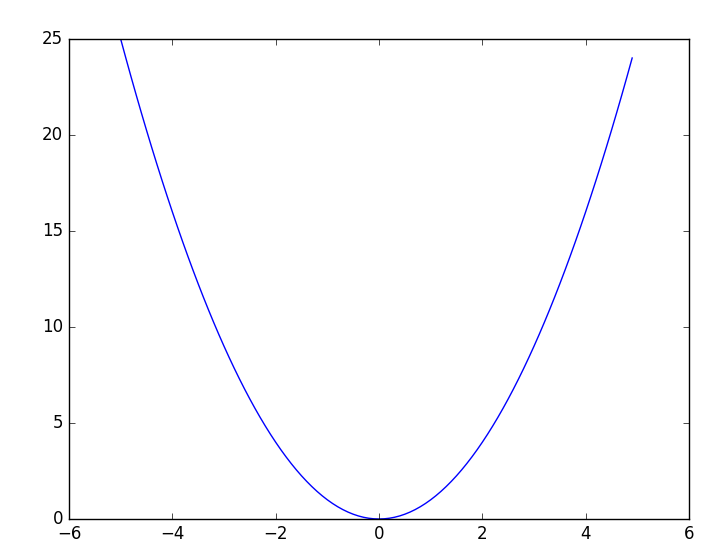
\includegraphics [width=7cm,height=7cm]{../pic/T1-1_func.png} 
\caption{$F(x) = (x-2.5)^2$图像}
\end{figure}
\indent 对于该问题,只要生成较为均匀的初始种群,经过若干代进化后则可以收敛到最小值点。\\
\indent 由于要找到最小值点,适应度函数应是关于目标值的减函数,本例中采用如下形式的适应度函数:
\begin{equation}
	fitVal=-ln(objVal+eps) \indent eps=1e-12
\end{equation}
\indent 在目标值后加上一个小量是为了避免在0点处超出定义域。由于问题较简单,因此不采用“精英”策略,即不保留当前种群中适应度最高的个体到下一代。

\subsection{编程实现}
本实验用C++实现,采用“面向对象”的方法,将“染色体”抽象为一个类,该类中包含了描述该条染色体信息的一些数据成员,并封装了交叉、变异操作。主函数中的流程如下:
\begin{figure}[htbp]\centering
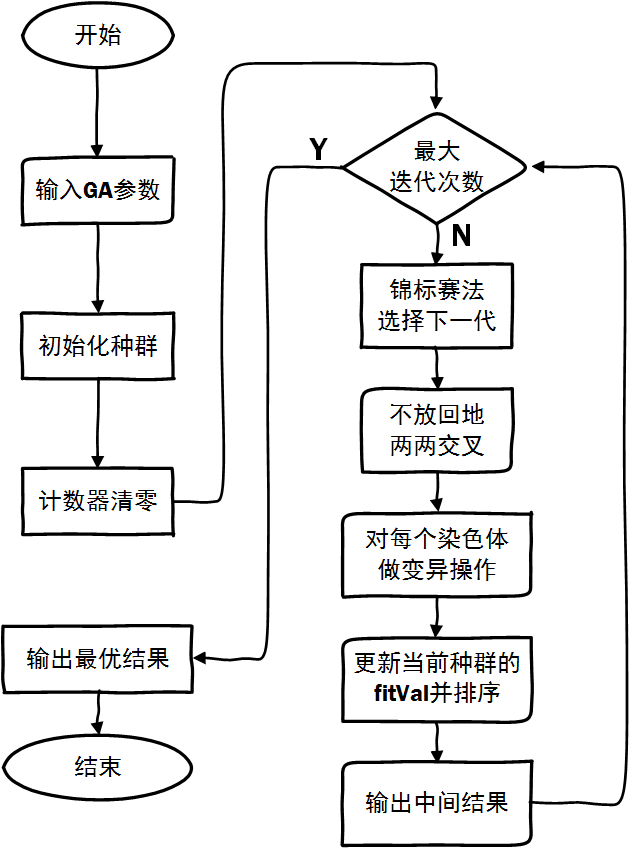
\includegraphics [width=9cm,height=13cm]{../pic/T1-1_procedure.png} 
\caption{GA求一元函数最小值程序流程}
\end{figure}

\indent 本实验的选择算子采用锦标赛选择法,每次有放回地随机选2个个体,然后取适应值高的个体复制到下一代留作进一步进化操作。虽然赌轮选择是较为常用的一种选择方法,但是其误差较大,因此本实验不采用。\\
\indent 交叉算子和变异算子封装在每个染色体对象中。交叉操作采用单点交叉的方式,每次随机选择一个交叉点,再根据给定的交叉概率(P\_Cross)决定是否执行交叉运算。\\
\indent 变异操作较简单,算子在遍历基因串的每一位时取一个随机概率,若该随机概率小于设定的变异概率(P\_Mutate)则反转(Flip)该位,否则保持不变。

\subsection{运行结果与分析}
本实验的参数取值如下:
\begin{table}[htbp]\centering
\begin{tabular}{cc}
  \toprule
  参数 & 值 \\
  \midrule
  基因串长度 & 24 \\
  自变量精度 & 5.96046e-007\\
  种群规模   & 200 \\
  迭代次数   & 80 \\
  交叉概率   & 0.65 \\
  变异概率   & 0.001 \\
  \bottomrule
\end{tabular}
\caption{GA求一元函数最小值测试参数}
\end{table}

\indent 得到的结果如下图所示:
\begin{figure}[htbp]\centering
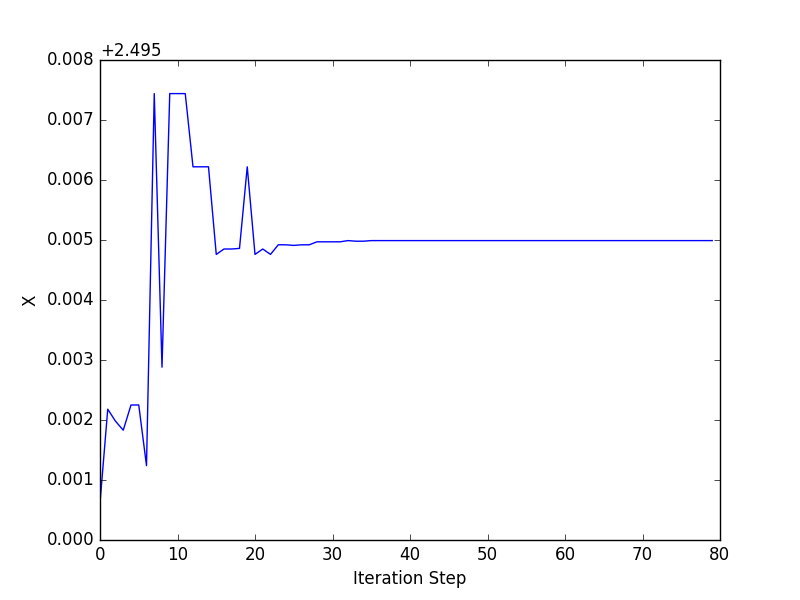
\includegraphics [width=8cm,height=8cm]{../pic/T1-1_res_x.png} 
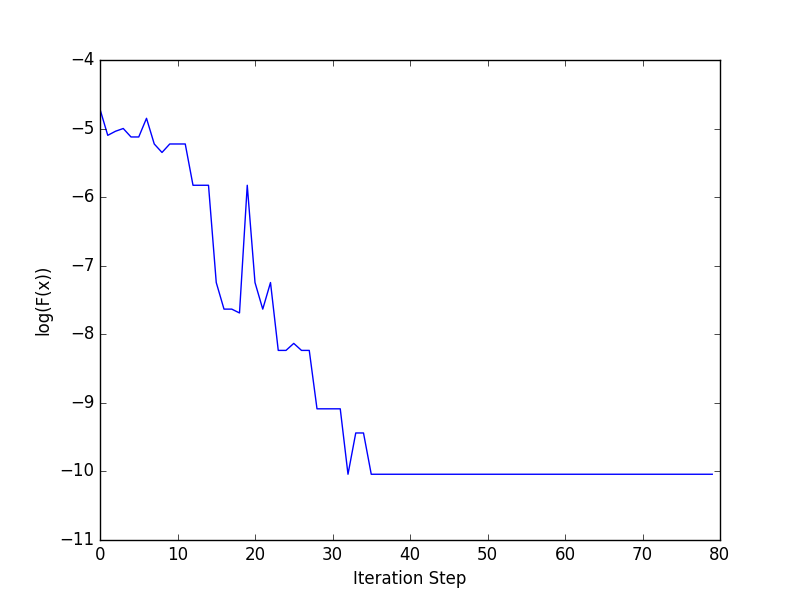
\includegraphics [width=8cm,height=8cm]{../pic/T1-1_res_fx.png} 
\caption{GA求一元函数最小值结果}
\end{figure}

\indent 可见对于简单的一元函数,遗传算法在给定区间上能够较快地收敛到极值点,虽然在初始阶段有振荡,但整体效果仍然较好。

\section{求二元函数最小值点}

\subsection{问题描述}
考虑如下优化问题:
\begin{equation}
	\min_{x_1,x_2} F(x_1,x_2) = (x_1-1.5)^4+(x_2+1.5)^2 \indent -3.0 \leq x_i \leq 3.0,i=1,2 
\end{equation}

\subsection{问题分析}
理论上,该二元函数取得其全局最优解0。该函数在给定区间上的图像如下:
\begin{figure}[htbp]\centering
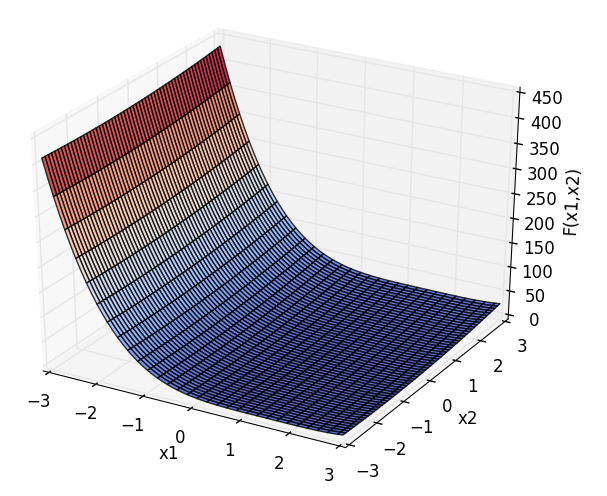
\includegraphics [width=11cm,height=11cm]{../pic/T1-2_func.png} 
\caption{$F(x_1,x_2) = (x_1-1.5)^4+(x_2+1.5)^2$函数图像}
\end{figure}

\indent 由于目标函数中有两个变量,因此情况较上一例略复杂,但原理相同,均是先生成较为均匀的初始种群,再经过若干代进化后收敛到最小值点。\\
\indent 虽然有两个变量,但是仍可以在一个基因串中表示,本实验的处理方法是用基因串的前半截表示第一个变量,用后半截表示另一个变量。\\
\indent 由于要找到最小值点,适应度函数应是关于目标值的减函数,本例中采用如下形式的适应度函数:
\begin{equation}
	fitVal=-objVal
\end{equation}

\indent 由于在实验中未发现明显得发散现象,因此仍然不采用“精英”策略。

\subsection{编程实现}
本实验中对染色体的抽象和上例类似,同样采用“面向对象的方法”将“染色体”抽象为一个类,该类中包含了描述该条染色体信息的一些数据成员,并封装了交叉、变异操作。3个遗传算子的具体实现如下:\\
\indent 选择算子采用锦标赛选择法(Tournament),每次有放回地随机选2个个体,然后取适应值高的个体复制到下一代留作进一步进化操作。\\
\indent 交叉算子和变异算子封装在每个染色体对象中。交叉操作采用单点交叉的方式,每次随机选择一个交叉点,再根据给定的交叉概率(P\_Cross)决定是否执行交叉运算。\\
\indent 变异操作较简单,算子在遍历基因串的每一位时取一个随机概率,若该随机概率小于设定的变异概率(P\_Mutate)则反转(Flip)该位,否则保持不变。\\
\indent 由于本例要处理两个变量,因此“染色体”类中还新加入了表示变量基因串长度的数据成员,并对构造函数、目标值函数和适应值值函数做了相应的修改。主函数的流程如下:
\begin{figure}[htbp]\centering
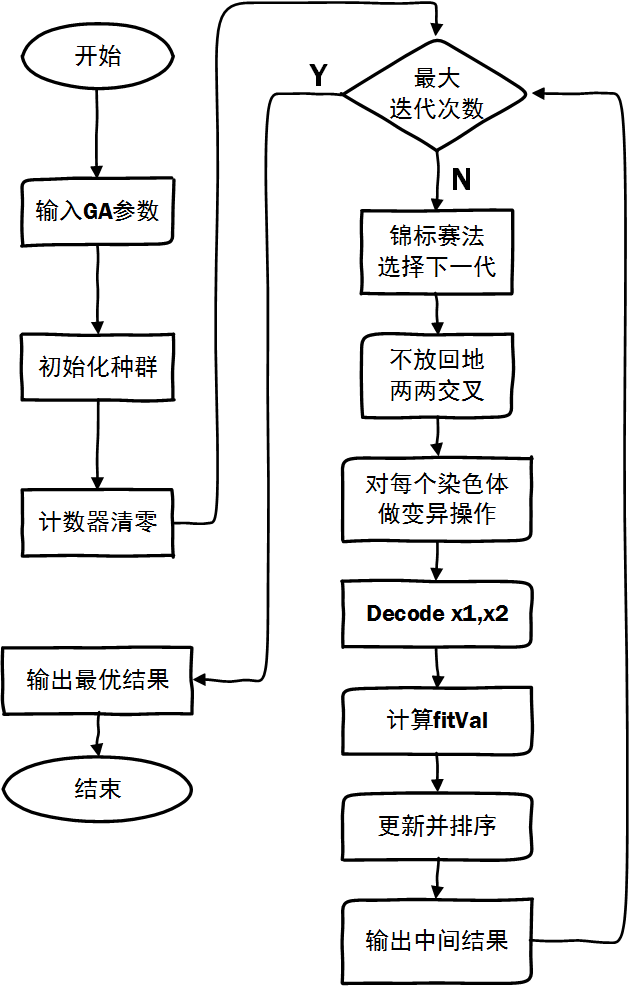
\includegraphics [width=8cm,height=11cm]{../pic/T1-2_procedure.png} 
\caption{GA求二元函数最小值程序流程}
\end{figure}

\subsection{运行结果与分析}
\indent 本实验的参数取值如下:
\begin{table}[htbp]\centering
\begin{tabular}{cc}
  \toprule
  参数 & 值 \\
  \midrule
  基因串长度 & 26 \\
  自变量$x_1$精度 & 0.000732422\\
  自变量$x_2$精度 & 0.000732422\\
  种群规模   & 200 \\
  迭代次数   & 80 \\
  交叉概率   & 0.65 \\
  变异概率   & 0.001 \\
  \bottomrule
\end{tabular}
\caption{GA求二元函数最小值测试参数}
\end{table}

\indent 得到的结果如下图所示:
\clearpage

\begin{figure}[htbp]\centering
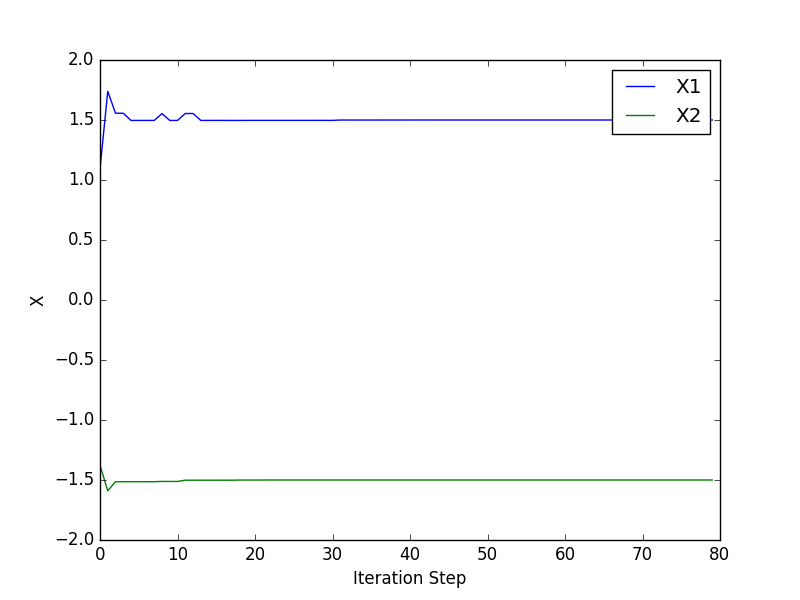
\includegraphics [width=8cm,height=8cm]{../pic/T1-2_res_x1_x2.png} 
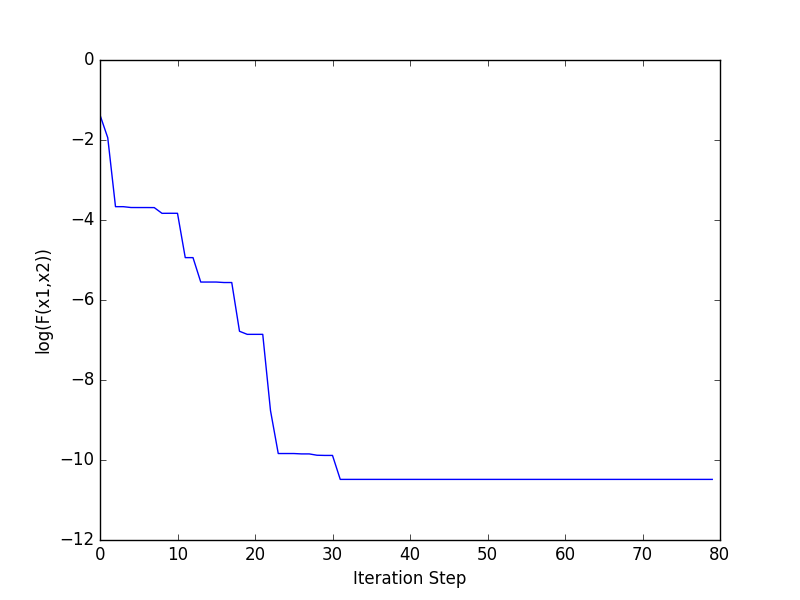
\includegraphics [width=8cm,height=8cm]{../pic/T1-2_res_f.png} 
\caption{GA求二元函数最小值结果}
\end{figure}

\indent 从实验结果可知,对于简单的二元函数,遗传算法在给定区间上也能够较快地收敛到极值点,没有早熟或振荡现象,效果较好。

\section{Nash GA求二元函数最小值点}

\subsection{问题描述}
Nash GA for minimization of $F(x,y)$ with 2 players:
\[ Player1=\min_x F(x,\overline{y})={\overline{y}}^2 (x-1)^2+(x \overline{y}-2)^4 \indent -4.0 \leq x \leq 4.0 \\ \]
\[ Player2=\min_y F(\overline{x},y)=y^2 (\overline{x}-1)^2+(\overline{x}y-2)^4 \indent -4.0 \leq y \leq 4.0 \\ \]

\subsection{问题分析}
这是一个二元函数,理论上,函数取得其全局最优解0。该函数在给定区间上的图像如下:
\begin{figure}[htbp]\centering
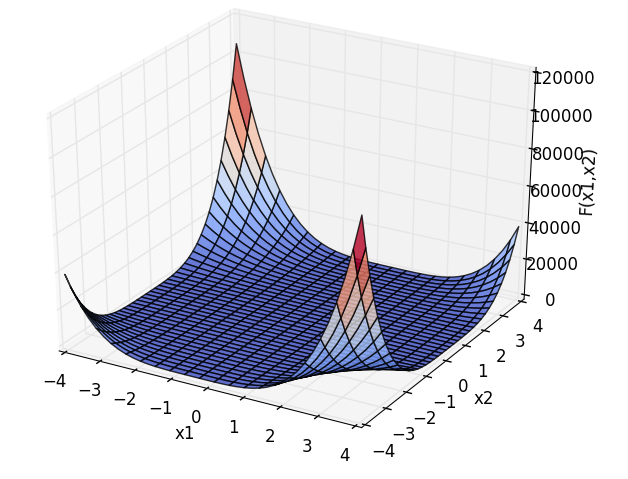
\includegraphics[width=5.5cm,height=5cm]{../pic/T2_func.png}
\caption{本例Nash GA的目标函数}
\end{figure}

\indent 该优化问题的处理方式和上一例处理二元函数的方法不同,Nash GA的做法是在每个迭代步中将2个变量分别交给2个Player来优化,每个Player根据对方的值来优化自己的值,最终达到所谓的Nash 均衡。而不是像上例中在一个迭代步中用1个GA同时优化2个变量。\\
\indent 算法的运行示意图如下:
\begin{figure}[htbp]\centering
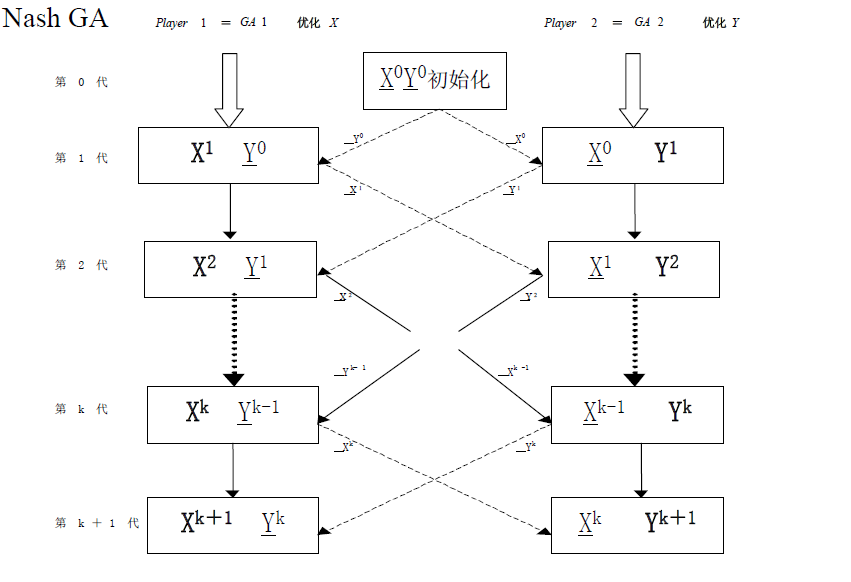
\includegraphics[width=14cm,height=10cm]{../pic/T2_illus.png}
\caption{Nash GA运行示意图}
\end{figure}

\indent 因此,该问题的解决思路是先从一个给定的初始值开始,然后针对每个变量分别运行一次针对一元函数的遗传优化算法,对每个变量都优化过后再将结果汇总,带入到下一个迭代步中。当达到指定的迭代次数后停止并输出。

\subsection{编程实现}
本实验既可用单线程程序实现也可以使用多线程程序实现。多线程程序意义明显,每一个线程对应一个玩家,初始时只需指定玩家编号,但在运行过程中要注意同步,两个玩家之间的要协调运行,防止出现data race或乱序。简单起见,本文只介绍单线程的程序。\\
\indent 为了便于调用,本例中将针对一元函数的遗传优化算法封装到一个函数中,这样在主函数中直接传入参数并调用即可。\\
\indent 另一个不同于前面两个程序的地方是自变量的管理,从可扩展性考虑,Nash GA算法可以用于多变量,因此求目标值的函数所接收的变量形式改为$std::vector<double>$,同时也便于动态增减元素,目标函数在染色体对象被构造时以函数指针的形式传入其中,如下所示:
\begin{lstlisting}
/*Definition of object function pointer*/
typedef double(*ObjFuncPtr)(const vector<double> &);
\end{lstlisting}

\indent 同时在染色体对象内部也用$std::vector<double>$来存储自变量,这样便统一了接口。
\clearpage

\indent 主函数的执行流程如下:
\begin{lstlisting}
Input();

for(size_t i=0;i<RoundCnt;i++)//Iteration
	for(size_t k=0;k<varCnt;k++)//Optimize each variable
		GA_Solver(F,local_var[k],k);

Output();
\end{lstlisting}

\indent 其中,$GA\_Solver$的定义如下:
\begin{lstlisting}
void GA_Solver(ObjFuncPtr func, vector<double> &var, size_t self);
\end{lstlisting}

\subsection{运行结果与分析}
\indent 本实验的参数取值如下:
\begin{table}[htbp]\centering
\begin{tabular}{cc}
  \toprule
  参数 & 值 \\
  \midrule
  基因串长度 & 26 \\
  自变量$x_1$精度 & 0.000732422\\
  自变量$x_2$精度 & 0.000732422\\
  种群规模   & 200 \\
  迭代次数   & 60 \\
  交叉概率   & 0.65 \\
  变异概率   & 0.001 \\
  \bottomrule
\end{tabular}
\end{table}

\indent 得到的结果如下图所示:
\begin{figure}[htbp]\centering
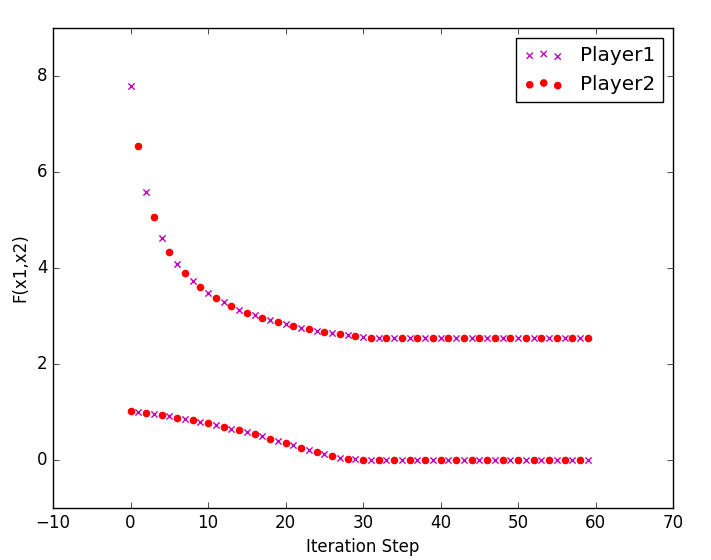
\includegraphics[width=9cm,height=8cm]{../pic/T2_res_f.png}
\caption{Nash GA优化二元函数结果}
\end{figure}

\indent 从实验结果可知,虽然给定的初始值是在一个局部最优的位置,但是Nash GA仍然能够将搜索范围拓展到全局并进而找到全局最优解$x=1,y=2$,两个Player交替落到最小值处,最终趋于稳定。虽然收敛的速度比起前两例慢了一些,但这揭示了一种多目标优化的方法,且利用Nash均衡处理得到的解空间具有一定的性质,同时具有理论和实践上的意义!

\section{程序运行说明}
直接运行src文件夹下对应的exe文件即可。\\
\indent 由于输出文件的路径在源码中是固定的,请保持文件结构,勿将exe文件移出src文件夹或修改其它文件夹!\\
\indent 若要编译源码,请使用支持C++11的编译器。对于Task2的多线程版本的程序,请确保编译器支持STL中多线程部分的头文件。

\section{总结}
本实验探究了遗传算法在函数优化中的应用,先用经典的遗传算法分别考察了针对一元函数和二元函数的优化问题,发现遗传算法能够较快地收敛到最优点,且没有早熟或振荡现象。\\
\indent 同时还探究了Nash GA,并用其处理了一个二元函数的优化问题,结果表明Nash GA同样能够获得相当好的收敛速度和精度,虽然在搜索方式上不同于经典的遗传算法,但是Nash GA同样具有全局搜索的能力,且搜索更具针对性,这为多目标优化问题提供了一种不一样的思路。

\end{document}
